\documentclass[a4paper, 11pt]{book}
\usepackage{/home/nora/Documents/Enseignement/Prepa/bpep/fichiers_utiles/preambule}
\usepackage{booktabs}

\makeatletter
\renewcommand{\@chapapp}{Kh\^olles MPSI -- semaine}
\makeatother
\renewcommand\thechapter{9}

% \toggletrue{corrige}  % décommenter pour passer en mode corrigé

\begin{document}

\chapter{Sujet 1\siCorrige{\!\!-- corrig\'e}}

\resetQ
\subimport{/home/nora/Documents/Enseignement/Prepa/bpep/exercices/Colle/cinetique_gazeuse/}{sujet.tex}

\newpage

\chapter{Sujet 2\siCorrige{\!\!-- corrigé}}

\resetQ
\subimport{/home/nora/Documents/Enseignement/Prepa/bpep/exercices/Colle/cinetique_chimique_2/}{sujet.tex}

\newpage

\chapter{Sujet 3\siCorrige{\!\!-- corrigé}}

\resetQ
\section{Intérêt de la dégénérescence de l'ordre}
On considère la réaction suivante~:
\[\ce{2Hg^{2+} + 2Fe^{2+} \longrightarrow Hg2^{2+} + 2Fe^{3+}}\]
On suit deux expériences à \SI{80}{\degreeCelsius} par spectrophotométrie. On
définit $\alpha = \DS \frac{[\ce{Hg^{2+}}]}{[\ce{Hg^{2+}}]_0}$.
\begin{description}
	\item[Expérience 1] : $[\ce{Fe^{2+}}]_0 = \SI{0.100}{mol.L^{-1}}$ et
		$[\ce{Hg^{2+}}]_0 = \SI{0.100}{mol.L^{-1}}$
		\begin{center}
			\begin{tabular}{lccccc}
				\toprule
				$t (\SI{e5}{s})$ &
				\num{0.0}        & \num{1.0}   & \num{2.0}   & \num{3.0}   & $\infty$ \\
				\midrule
				$\alpha(t)$      &
				\num{1.000}      & \num{0.500} & \num{0.333} & \num{0.250} &
				\num{0.000}                                                           \\
				\bottomrule
			\end{tabular}
		\end{center}
	\item[Expérience 2] : $[\ce{Fe^{2+}}]_0 = \SI{0.100}{mol.L^{-1}}$ et
		$[\ce{Hg^{2+}}]_0 = \SI{0.001}{mol.L^{-1}}$
		\begin{center}
			\begin{tabular}{lcccccc}
				\toprule
				$t (\SI{e5}{s})$ &
				\num{0.0}        & \num{0.5}   & \num{1.0}   & \num{1.5}   & \num{2.0} &
				$\infty$                                                                 \\
				\midrule
				$\alpha(t)$      &
				\num{1.000}      & \num{0.585} & \num{0.348} & \num{0.205} &
				\num{0.122}      & \num{0.000}                                           \\
				\bottomrule
			\end{tabular}
		\end{center}
\end{description}

\QR{On considère que la réaction est d'ordre partiel $p$ par rapport à
$\ce{Fe^{2+}}$ et $q$ par rapport à $\ce{Hg^{2+}}$. Écrire
l'expression de la vitesse de réaction.}
{
Par définition,
\[\boxed{v = k[\ce{Fe^{2+}}]^p[\ce{Hg^{2+}}]^q}\]
}

\QR{
Déterminer l'ordre global de la réaction à l'aide de l'expérience 1.
}{
Avec les proportions stœchiométriques, on a $[\ce{Fe^{2+}}] =
	[\ce{Hg^{2+}}]$, et par définition de $\alpha$ on a $[\ce{Hg^{2+}}] =
	\alpha[\ce{Hg^{2+}}]_0$. Ainsi,
\begin{gather*}
	v = k \left( \alpha [\ce{Hg^{2+}}]_0\right)^{p+q}
	\Leftrightarrow
	v = k' \alpha^{p+q}
\end{gather*}
avec $k' = k[\ce{Hg^{2+}}]_0{}^{p+q}$. On remarque que $\alpha$
évolue de manière inversement proportionnelle au temps, ce qui
correspond à une cinétique d'ordre 2 (par méthode intégrale). On a donc
\[\boxed{p+q = 2}\]
}

\QR{
	Déterminer $q$ à l'aide de l'expérience 2. En déduire $p$.
}{
	Avec un large excès d'ions fer II, on se place dans l'approximation de
	la dégénérescence de l'ordre, c'est-à-dire que $\forall t\quad
		[\ce{Fe^{2+}}] \approx [\ce{Fe^{2+}}]_0$. Ainsi,
	\begin{gather*}
		v = k_{\rm app} \left( \alpha [\ce{Hg^{2+}}]_0 \right)^q
		\qavec
		k_{\rm app} = k [\ce{Fe^{2+}}]_0{}^p
	\end{gather*}
	Étant donné que $p+q = 2$, ni l'un ni l'autre ne peut être plus grand
	que $2$. De plus, si $p=0$, alors $k_{\rm app} = k$ et la cinétique
	n'aurait pas changé~: on suppose donc que $p=1=q$ et on teste cette
	hypothèse avec les données de l'expérience 2. Pour cela, on écrit la
	relation entre la vitesse de la réaction et la concentration en ions
	mercure et on exprime la solution de l'équation différentielle obtenue~:
	\begin{gather*}
		v = - \frac{1}{2} \diff{[\ce{Hg^{2+}}]}{t} = k_{\rm app} [\ce{Hg^{2+}}]
		\Rightarrow
		[\ce{Hg^{2+}}] = [\ce{Hg^{2+}}]_0 \exr^{-2k_{\rm app}t}\\
		\Leftrightarrow
		\boxed{
		\alpha = \exr^{-2k_{\rm app}t}}
	\end{gather*}
	On vérifie cette hypothèse en traçant $\ln \alpha = f(t)$, soit
	en faisant la régression linéaire
	\[y = ax
		\qavec
		\left\{
		\begin{array}{rcl}
			y & = & \alpha        \\
			a & = & -2k_{\rm app} \\
			x & = & t
		\end{array}
		\right.
	\]
	\begin{minipage}{0.45\linewidth}
		On trouve ici aussi une droite avec un coefficient de corrélation
		$r^2 = \num{0.99997}$, confirmant que l'ordre partiel en mercure est
		compatible avec 1~: \fbox{$q=1$}. Comme $p+q=2$, on a forcément
		\fbox{$p=1$}.
	\end{minipage}
	\hfill
	\begin{minipage}{0.55\linewidth}
		\begin{center}
			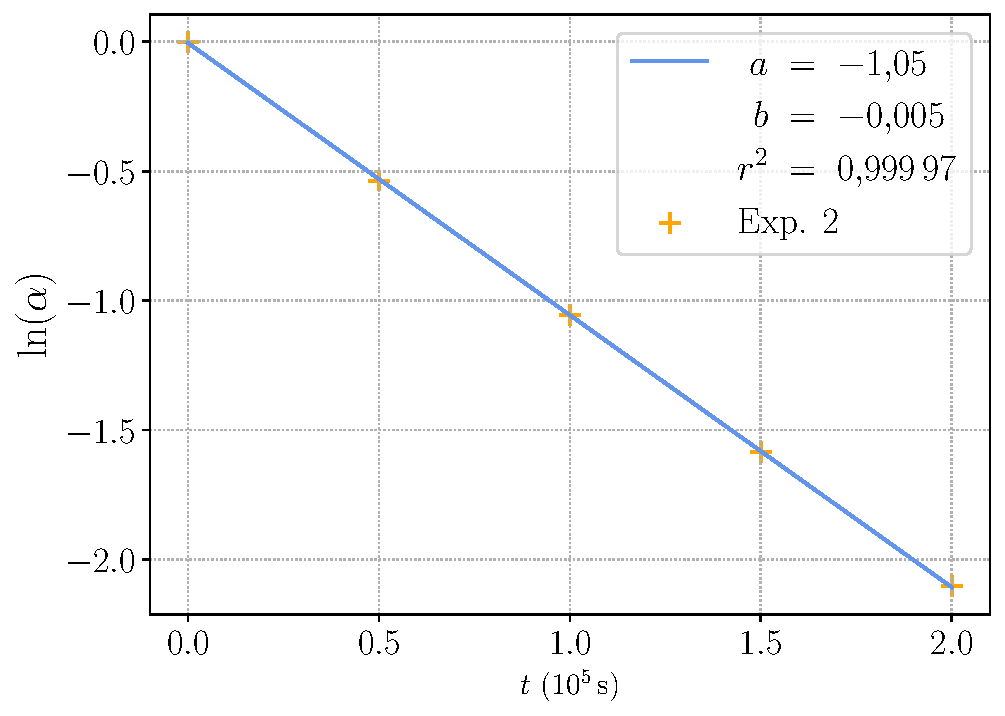
\includegraphics[width=\linewidth]{exo6_a1}
		\end{center}
	\end{minipage}
}

\QR{
	Déterminer la constante de vitesse de la réaction.
}{
	On obtient la constante de vitesse grâce à la pente de la régression
	linéaire~:
	\begin{gather*}
		-2k_{\rm app} = -2 k[\ce{Fe^{2+}}]_0
		\Leftrightarrow
		\boxed{
			k = \frac{2k_{\rm app}}{2[\ce{Fe^{2+}}]_0}}
		\qavec
		\left\{
		\begin{array}{rcl}
			2k_{\rm app}     & = & \SI{1.051e-5}{s^{-1}}  \\\relax
			[\ce{Fe^{2+}}]_0 & = & \SI{0.100}{mol.L^{-1}}
		\end{array}
		\right.\\
		\mathrm{A.N.~:}\quad
		\boxed{k = \SI{5.3e-5}{mol^{-1}.L.s^{-1}}}
	\end{gather*}
}

\end{document}
